\chapter{Shakarr's Vanishing Mansion}
\DndDropCapLine{T}{he adventurers arrive in Garon City,} hopefully prepared for battles with animated objects, encounters mysterious wizards with troubled pasts, and a town full of people who will range from curious to hostile. 
\section{Background}
The party should come into Garon City as a group of Level 2 adventurers after dealing with the smuggling ring in Geranium Village in the previous chapter. If they avoided fights or did not gain enough XP to reach Level 2, the party should be given a few random encounters on the road between Geranium Village and Garon City, before attempting to enter the Mysterious Mansion.\\
The party should be looking to find the mysterious wizard who recently appeared in town, to see if he has any insights into the unique Brand of Amberia Friggsdottir. This wizard is actually Shakarr, human representative on the Council of Seven. Shakarr is very powerful, but his mind has been addled by a spell that went wrong a long time ago. Malmalor Lumena, tiefling widow of Malvol Lumena who was betrayed and murdered at the Compact of the Seven Races (see Chapter~\ref{Kiraki}, disguised herself and befriended Shakarr.\\
Shakarr was obsessed with chronological magic, and trying to invent a spell that could send him through time as he pleased. Malmalor sabotaged his spell circle, and when he tried to execute the spell it backfired, and scrambled his mind; his mind sometimes appears to be from a different point in time, either lacking memories he should have, or sometimes gifted with foresight. Rarely is his mind in the present moment. \\
Malmalor then set about making sure he was elected to be the Mayor of Gold City, and therefore the human representative on the Council of Seven, replacing Talus Cherry. Due to his mental state, he is infuriatingly incompetent, and often makes votes against the best interests of his allies. However, he keeps getting reelected, as Malmalor laced his skin with a type of mushroom, the spores of which cause people to forget about his incompetence.\\
Another side effect of his temporal spell, Shakarr was given a protracted life, living now for over four hundred years. Now, in a paranoid state, he has fled Gold City and arrived in Garon City, with an entire magical mansion in tow. The people of Garon City are nervous about the sudden appearance of the mansion, and the animated objects within. Townsfolk who went to greet the newcomer were chased away by magical brooms and armor.
\section{The City}
Garon City is a bustling town of population 3,500 in central Kiraki. The lands to the west and south are mostly farmland, whereas to the north and east the farmland eventually gives way to thick forest.\\
The town is populated by a mix of all of the races protected by the Compact of the Seven Races, though humans, elves, and arboreans are most common, and seafolk are quite rare. The has a fairly young history, it sprung up after the Compact of the Seven Races, and has steadily grown as a place of rest and restocking in the busy trade route between Gold City and Illithium City. The oldest part of the city surrounds the town's biggest attraction: \textbf{The Shrine of the Sun}, a monument to Taranis. \\
\section{Points of Interest}
The town is big enough to have most amenities that a traveling adventurer might need, such as a blacksmith, an armorer, a large general store, an inn, and more. This section lays out some of the more interesting ones, leaving the rest up to the DM's discretion.
\subsection{The Tallyfoot Inn}
For many adventurers, the first stop in any town is an inn. There are two places to stay in Garon City. Borna's Tallyfoot inn is the one accessible to the average traveler, though there is also the Council Station, for those with more money to spend or for those of political importance.\\
The Tallyfoot is a standard tavern and inn, a large white-painted building on the west end of town. There are twelve rooms at the inn, and they go for standard rates. The downstairs tavern is a popular place among both travelers and locals. 
\subsubsection{Borna Bestwick and Family}
Borna is the inn's owner and keeper. She is a stocky human woman in her late 40s, with wavy brown hair that is beginning to gray. She is polite, but not particularly talkative. Her family lives with her at the Inn. Her sons Benny and Tenson, as well as her husband Rigor, are all very invested in the local branch of the Cult of The Sun. If they hear any ill spoken of Taranis, they will be upset.
\subsubsection{Aca, Arva, and Aida}
Three dwarven women are patrons of the tavern. Aca is short, bearded, and canankerous. Arva is average height for a dwarf, clean shaven, and boisterous and flirty. Aida is almost human height, with golden long hair, and probably the most beautiful dwarf by human standards anyone in the party has ever seen. She is quiet and sad. If the party approaches, they will ask the party if they have any news from Illithium City, as they have family there and are worried about the war with the orcs. They might offer a small reward (2d4 gold) for information. The
\subsubsection{Sacrave Lumena} The same hooded figure who was present at the Inn in Geranium Village can be spotted here one evening. Like in Geranium Village, if approached, the figure will pull their cloak tighter and ignore the attention. The tiefling is desperate to keep their identity secret, as tieflings are not welcome in Kiraki. The most information the players might get out of her by normal means is that she is on an errand for Ignotius Cherry.
\subsection{The Guards' Garrison}
\subsection{The Barnyards}
\subsection{The Shrine of the Sun}
\subsection{The General Store}
Kako, a half-elf woman with long dark hair and a star shaped earring, runs Garon City's general store. She is welcoming, and has most common adventuring gear as well as food.

\section{Overarching Narrative Connections}
In Garon City, the players can learn of the devout worship of Taranis by the Cult of the Sun, how the general populace is uneasy about the war with the orcs, and through the Mysterious Mansion adventure, learn tidbits about the history of Shakarr and his experiments with time.

\section{Adventure Summary}
A Mysterious Mansion appeared on a hillside just outside of town about a month before the party gets there. A few people who went to investigate it were chased away by animated furniture. The mansion is rumored to be the home of a powerful wizard, and given the mysterious circumstances of its arrival, 
\section{Adventure Hooks}
\subsection{Cherry's Request}
If the players did the first adventure in this book, they should have been told by Ignotious Cherry that they should seek out some knowledgeable wizards to help decipher the meaning of Amberia Friggsdottir's brand. One of his suggested wizards is the rumored wizard inhabitant of the Mysterious Mansion.
\subsection{A Child's Curiosity}
While walking the streets of town, a curious human boy named Davy will follow them. He can be caught and questioned, and reveals he really wants some adventurers to check out the mansion because his uncle Frank, a guardsman was apparently too scared. If they go talk to Frank, they can learn he was attacked by animated furniture, giving them an eye to be wary in the Grand Foyer of the Mansion.
\section{The Mysterious Mansion}
\subsection{Location in Town}
The Mysterious Mansion is located at the northeast end of town, on a hill that looks out over the whole town. The mansion is visible from nearly everywhere in town, as it seemingly looms over the residents below.
\subsection{The Exterior}

\subsection{The First Floor}
The following locations are identified on Map~3.1.
\subsubsection{1. Grand Foyer}
\begin{DndReadAloud}
  As you enter the front doors to the mansion, a grand foyer stretches before you. The foyer is adorned with fine drapes in the colors of Kiraki (maroon, cobalt, and yellow, and sun-glow yellow). A grand carpet lines the floor from the entrance. Fine statues and suits of armor line the walls. Four great pillars hold up the high (20 feet.) ceiling.\\
  At the end of the entrance hall stands a lone figure. An elderly human man, with a long white beard and a pocket watch on a chain around his neck. Upon seeing you enter, he exclaims, "Oh, I think I know why you've come!" He then immediately turns around and makes a run for it out through the back right door of the foyer.
\end{DndReadAloud}
In the entrance hall, the players gain a glimpse of Shakarr, the human Representative on the Council of Seven. They will likely not learn his identity until much later, as he upon seeing them immediately flees. Any attempts by the party to cast a spell to restrain him is met with a 6th level counterspell.\\
As he leaves the room, Shakarr should snap his fingers, and the moment any of the party step onto the grand carpet in the center of the room, they are embroiled into battle, as the carpet comes alive as a \textbf{Rug of Smothering}, and two of the six suits of armor come to life as \textbf{Animated Armor}.\\
\subparagraph{Secret Door} A secret door lies behind one of the normal suits or armor on the left. A DC~13 Intelligence (Investigation) check can be made to find the secret door. The door is locked, but can be opened with a successful DC~13 Dexterity check with Thieves' tools, or a DC~15 Strength check to brute force it open.
\subparagraph{Hidden Closet} At the end of the foyer, with an Intelligence (Investigation) check of DC~10 or higher, the party can notice an obscured servant's door, which fits seemlessly into the wall.
\subsubsection{2. Hallway}
\begin{DndReadAloud}
  The room you enter is a narrow hallway. It is well kept and lit. There are two doors at the far end of the hallway leading opposite directions. 
\end{DndReadAloud}
An otherwise empty hallway, the party can with a DC~17 Wisdom (Perception) check hear footsteps running up stairs in the room to the north.
\subsubsection{3. Hidden Closet}
\begin{DndReadAloud}
  The room appears to be a dusty, rarely used servants' supply closet. There are brooms, mops, and other cleaning tools, and a big pile of white linen sheets. 
\end{DndReadAloud}
\subparagraph{Treasure} With a successful DC~11 Intelligence (Investigation) check of the room, the party can find a chest buried under a pile of white sheets. The chest, which is unlocked contains 10d10 silver pieces and 4d10 gold pieces.
\subsubsection{4. Arboretum}
\begin{DndReadAloud}
  The room is a steamy arboretum. Giant windows edge the west and south sides of the room, filling the room with light. Plants of exotic varieties fill the room. Lush potted trees and plants obscure your view of the full room. As you enter, a light, bitter smelling mist from a small hole in the ceiling drifts over you and humidifies the plants.
\end{DndReadAloud}
In this room, a \textbf{Violet Fungus} lurks, waiting to attack the careless adventurer. It can be identified from afar before attacking with a DC~14 Intelligence (Nature) check.\\
At the far south of the room, a \textbf{Giant Poisonous Snake} menaces from the branches of a potted tree.\\
\subparagraph{Development}
The clever player might put together that the mists from the small hole above them corresponds to the location as Shakarr's toilet and bathroom on the floor above.
\subparagraph{Treasure} A perceptive adventurer might find the soil of one of the plants recently disturbed. With a DC~13 Intelligence (Investigation) check, a player can notice this, and dig up a \textbf{Charm of Darkvision}.\\
If the players ask if any of the plants can be harvested for materials, a Wisdom (Survival) check can be made, and on a score of 16 or above the players can identify enough herbs and plants to gather materials for anyone proficient with an herbalism kit to create a \textbf{Potion of Healing}. On a score of 20 or above, the players can identify a bunch of three \textbf{Fruits of Forgetting}, one of Merope's four \textbf{Sacred Fruits} (see Chapter~\ref{Items}).
\subsubsection{5. Grand Stairway}
\subparagraph{Development}
If the players broke in through a window in the arboretum rather than using the main entrance, the scene where Shakarr is encountered happens in this room, rather than the Grand Foyer. He is at the top of the stairs, and activates two more \textbf{Animated Armor} to his defense. Otherwise, the players can hear pattering footsteps at the top of the stairs. The armors still attack in this case.
\begin{DndReadAloud}
  A grand staircase rises to the second floor. To the sides of the stairs, two suits of armor stand tall. A closed door is present on the far side of the room.
\end{DndReadAloud}
\subsubsection{6. Basement Stairwell}
\begin{DndReadAloud}
    The room is eerily empty, save for a set of stone stairs descending into the earth, and another door at the south-west corner of the room.
\end{DndReadAloud}
Here, there are stairs that lead to the basement. These stairs will still be here after Shakarr causes the rest of the mansion to vanish.
\subsubsection{7. Dining Hall}
\begin{DndReadAloud}
    A grand dining hall that does not appear to have been used for a long while. One of the chairs is overturned. A sheen of dust coats the table.
\end{DndReadAloud}
This room appears devoid of interest, but a successful DC~15 Intelligence (Investigation) check will reveal that the overturned chair is directly beneath a panel in the ceiling leading to an attic crawlspace. If the party stacks some chairs and stands on them, a Strength (Athletics) check of DC~12 can be attempted to do a pull-up into the crawlspace.
\subparagraph{Treasure} The silverware is genuine silver, and can be collected and is worth a total of 6 gold.
\subsection{The Second Floor}
If the players come to the second floor before finishing exploring the first floor, they may lose out on the chance later. Because of this, the Dungeon Master may choose to place Shakarr in whichever of the rooms on the second floor that the players visit last, or in the room of their choice. Upon finding Shakarr, he will squeak in panic, snap his fingers, then disappear.\\
When he does this, the mansion around them will begin to shimmer and become transparent, and they will only have 6d10 more seconds to explore or return to the first floor before the mansion and everything in it disappears, and the players fall to the first floor twenty feet below. When the mansion disappears, all treasures, intel, and monsters not already in their possession or battled from the first or second floor disappear forever. All that remains is a ruined foundation and the basement (with everything still in it). The stairs for the basement will now be overgrown with plants, and the players should succeed on a DC~10 Intelligence (Investigation) check to find it.
\subsubsection{8. Upstairs Stairwell}
\begin{DndReadAloud}
    You emerge into an empty room at the top of the grand stairs. A door is slowly swinging closed at the south east corner of the room.
\end{DndReadAloud}
A room which contains stairs back down to the first floor.
\subsubsection{9. Upstairs Hallway}
\begin{DndReadAloud}
    A hallway stretches ahead. There are three doors besides the one you came through on the right, and halfway down, the hallway branches off to the left.
\end{DndReadAloud}
This hallway connects directly to the study, there are no doors blocking view of the study.
\subsubsection{10. Bedroom 1}
\begin{DndReadAloud}
    The room appears to be a simple guest bedroom. There is a bed and a small set of drawers.
\end{DndReadAloud}
If a player opens the drawers, they find a set of papers. On the set of papers, the words appear blurry. A player must make a successful DC~16 Intelligence (Arcana) check to read the magic words ``malus avis.'' The papers transform into a flock of \textbf{Paper Birds} and attack.
\subparagraph{Development} If the players speak the magic words, peacefully ending the enchantment, or destroy the \textbf{Paper Birds} in a way that leaves them mostly intact (no slashing, piercing, acid, fire or radiant damage), the players can read some notes from the birds.
\begin{DndReadAloud}
    \textit{Merorise 4th, 7 PCS} (DM note, see Chapter\ref{Kiraki}.\ref{Year})\\
    \textit{The master had a visitor today. A druidic woman stopped by and offered to help him with his experiments. I don't trust her, I think she has ulterior motives.}\\
    \textit{Merorise 6th, 7 PCS\\
    The master has changed. Sometimes he knows not who I am, and sometimes, he laments my death which he claims he has forseen.}
\end{DndReadAloud}
The entries foreshadow the reveal of Malmalor Lumena's curse, and her disruption of Shakarr's spell that scrambled his mind. If you didn't already read the section on the current year in Kiraki, it might be a good idea to read that section of Chapter~\ref{Kiraki} so that you are familiar with how long ago this letter was written.
\subsubsection{11. Bedroom 2}
\begin{DndReadAloud}
    The room appears to be (another) simple guest bedroom. There is a bed and a small set of drawers.
\end{DndReadAloud}
\subparagraph{Treasure} In one of the drawers, 12~gold worth of jewelry and knick-knacks can be found.
\subsubsection{12. Bedroom 3}
\begin{DndReadAloud}
    The room appears to be (another) simple guest bedroom. There is a bed and a broom laying against the wall.
\end{DndReadAloud}
Upon entering the room, the bedsheets and broom will attack as \textbf{Angry Bedsheets} (see Chapter~\ref{Monsters}) and an \textbf{Animated Broom}.
\subsubsection{13. Master Bedroom Antechamber}
\begin{DndReadAloud}
    The room appears to be an antechamber to a masterbedroom. There is an open door to a bathroom, a closed door, and an ottoman upon which some robes are stacked.
    \end{DndReadAloud}
    \subparagraph{Treasure} If the party looks closer at the ottoman, they can find it opens, and inside is a necklace with a diamond valued at 15 gold pieces.
\subsubsection{14. Master Bathroom}
    \begin{DndReadAloud}
    The room is a bathroom, with a simple washbasin, and a toilet.
    \end{DndReadAloud}
    By peering into the toilet, the party can see the arboretum below. If they did not kill the \textbf{Giant Poisonous Snake} earlier, it comes out of the toilet and attacks.
\subsubsection{15. Master Bedroom}
\begin{DndReadAloud}
    The master bedroom. A king sized bed spans the room. The bed is unmade, and there is no evidence that it has recently been attended to by any servants.
    \end{DndReadAloud}
    \subparagraph{Development} If this is the last room that the players have to explore on the second floor, they should place Shakarr in here. He will act as in the description at the beginning of the second floor. Otherwise, if the players come here early on, he can be instead located in the Study or one of the guest bedrooms, or even back on the first floor.
\subsubsection{16. Attic Crawlspace}
\begin{DndReadAloud}
    You've pulled yourself into a dusty, dimly lit crawlspace with a 4 foot high ceiling. A large beam supports the structure in the middle of the room.
    \end{DndReadAloud}
This room is only accessible if the players found the ceiling panel in the dining hall below, or if they perform some kind of spell with area of effect damage that punches a hole in the hallway wall.
\subparagraph{Treasure}In the crawl space, there is a chest with one finely crafted pocket watch for each player. Each watch can be sold for 100 gold. If an \textbf{Identify} spell is used on the watches, they will learn they have are \textbf{Shakarr's Pocketwatches} (see Chapter~\ref{Items}).
\subsubsection{17. Study}
\begin{DndReadAloud}
    You enter a room which is clearly a study. The room is well lit, and inviting. A desk is littered with papers.
    \end{DndReadAloud}
    \subparagraph{Development} Like the Master Bedroom, this may be the last room the players explore, and thus should be met with Shakarr as described at the beginning of the Second Floor. \\
    Otherwise, if the players inspect the desk they can find lots of notes. With a successful DC~14 Intelligence (Investigation) check, they can find that most of the papers are notes on spells about time. They also find a paper that reads: ``\textit{Must get this to the other members of the Council of Seven ASAP}.''
    \subparagraph{Treasure}
    They can find a \textbf{Wand of Scowls}, and if they have a wizard in the party, a spell book that contains the spells \textit{Detect Magic}, \textit{Identify}, and \textit{Unseen Servant}.
    
\subsection{The Basement Ruins}
The basement can be accessed before or after the mansion vanishes. 
\subsubsection{18. First Chamber}
\begin{DndReadAloud}
    You descend the stone stairs and the air becomes stale and humid. Beyond the base of the stairs, natural light quickly becomes a scarce resource. You enter an oddly shaped room with stone wall, and a ceiling about 8 feet high. The ground is a dusty packed soil. There is a door at the east end of the room, with some rubble on the ground in front of it.
\end{DndReadAloud}
The rubble covers a pit trap directly in front of a door, which the players must observe with a successful DC~14 Intelligence (Investigation) check. If they fail to spot it, the first one to step on the pit must make a DC~14 Dexterity Saving throw, or fall into a 12 feet deep spiked pit and take 2d6 piercing damage, and figure out a way to escape.
\subsubsection{19. Experiment Chamber}
\begin{DndReadAloud}
    You enter a very large, dark room more than 60 feet across. In the middle of the chamber, there are the chalk etchings of some kind of advanced spell circle. There are two other doors out of the room, to the north, and to the south-west.
\end{DndReadAloud}
The party can make a DC~13 Intelligence (Arcana) check to recognize this as a very advanced spell circle. If they have proficiency with arcana, you might also tell them that while the spell is too complicated for them to understand fully, they recognize that it has something to do with time, and also that it appears to not have successfully completed.\\
If the party comes back here at a later date when they can cast 5th or higher level spells, they can attempt to complete the ritual. The player attempting it should be warned it is very dangerous. The player should make an Intelligence (Arcana) check, an on a value of 10 or below, they suffer the same fate as Shakarr, and have their memories scrambled in time, only curable by a Wish spell. On a value of 11 to 15 they are booted 1d10 weeks into the future. On a value of 16 to 20 the spell circle permanently breaks and nothing else happens. Above a 20, and the spell circle will create a \textbf{Scroll of Time Stop}.
\subparagraph{Treasure} A player with a Wisdom (Perception) check of DC~12 might notice a broken sword against the back wall. This is a broken \textbf{+1 Greatsword} which can be fixed at a blacksmith.
\subsubsection{20. Wine Cellar}
\begin{DndReadAloud}
    The room ahead is dank and damp. Casks of old wine line the northern wall of the room. You hear squeaking, and you see the glitter of eyes beneath a sewer grate.
\end{DndReadAloud}
If the players proceed into this room, they are met with an angry \textbf{Swarm of Rats.}
\subparagraph{Treasure} If the players have any wineskins, they can fill them with a very finely aged wine from year 365 PCS. If they are clever enough to try and sell the entire barrels, they are worth 30 gold each, and there are six of them. If the players inspect the sewer grate, on a DC~18 Wisdom (Perception) check, they might hear the faintest whisper from the depths: ``The aberroth rise!''
\subsubsection{21. Trapped Chamber}
Upon opening the door and stepping into the room, the first party member must make a DC 16 Dexterity saving throw against an arrow trap aimed at the doorway, on a failure taking 2d6 piercing damage, and half as much on a pass. This trap could be spotted with a DC 19 Intelligence (Investigation) check, and disarmed with a DC 16 Dexterity check with \textbf{thieves' tools}.
\begin{DndReadAloud}
  Beyond the trap, the large chamber is inhabited by two giant toads. Against the back rocky wall, a pool of water runs along the ground.
\end{DndReadAloud}
The party must figure out how to deal with two \textbf{Giant Toads}. If they move slowly and act quietly, the toads will leave them alone.
\subparagraph{Secret Door}On a DC~15 Intelligence (Investigation) check, an adventurer can notice a point where the water runs into the rocks, and find the outline of a secret rocky door, which can be pushed open.
\subsubsection{22. Treasure Chamber}
\begin{DndReadAloud}
  Advancing through the hidden door, you see a room with two large chests sat against the western wall.
\end{DndReadAloud}
In the final basement chamber is a chest with the big reward for the dungeon, and a decoy chest which is actually a \textbf{Mimic}.
\subparagraph{Treasure}
Inside the chest is 20d10 gold, 20d10 silver, 3d10 copper, and a \textbf{Potion of Speed}. The mimic coughs up an additional 15 gold.
\begin{figure*}
  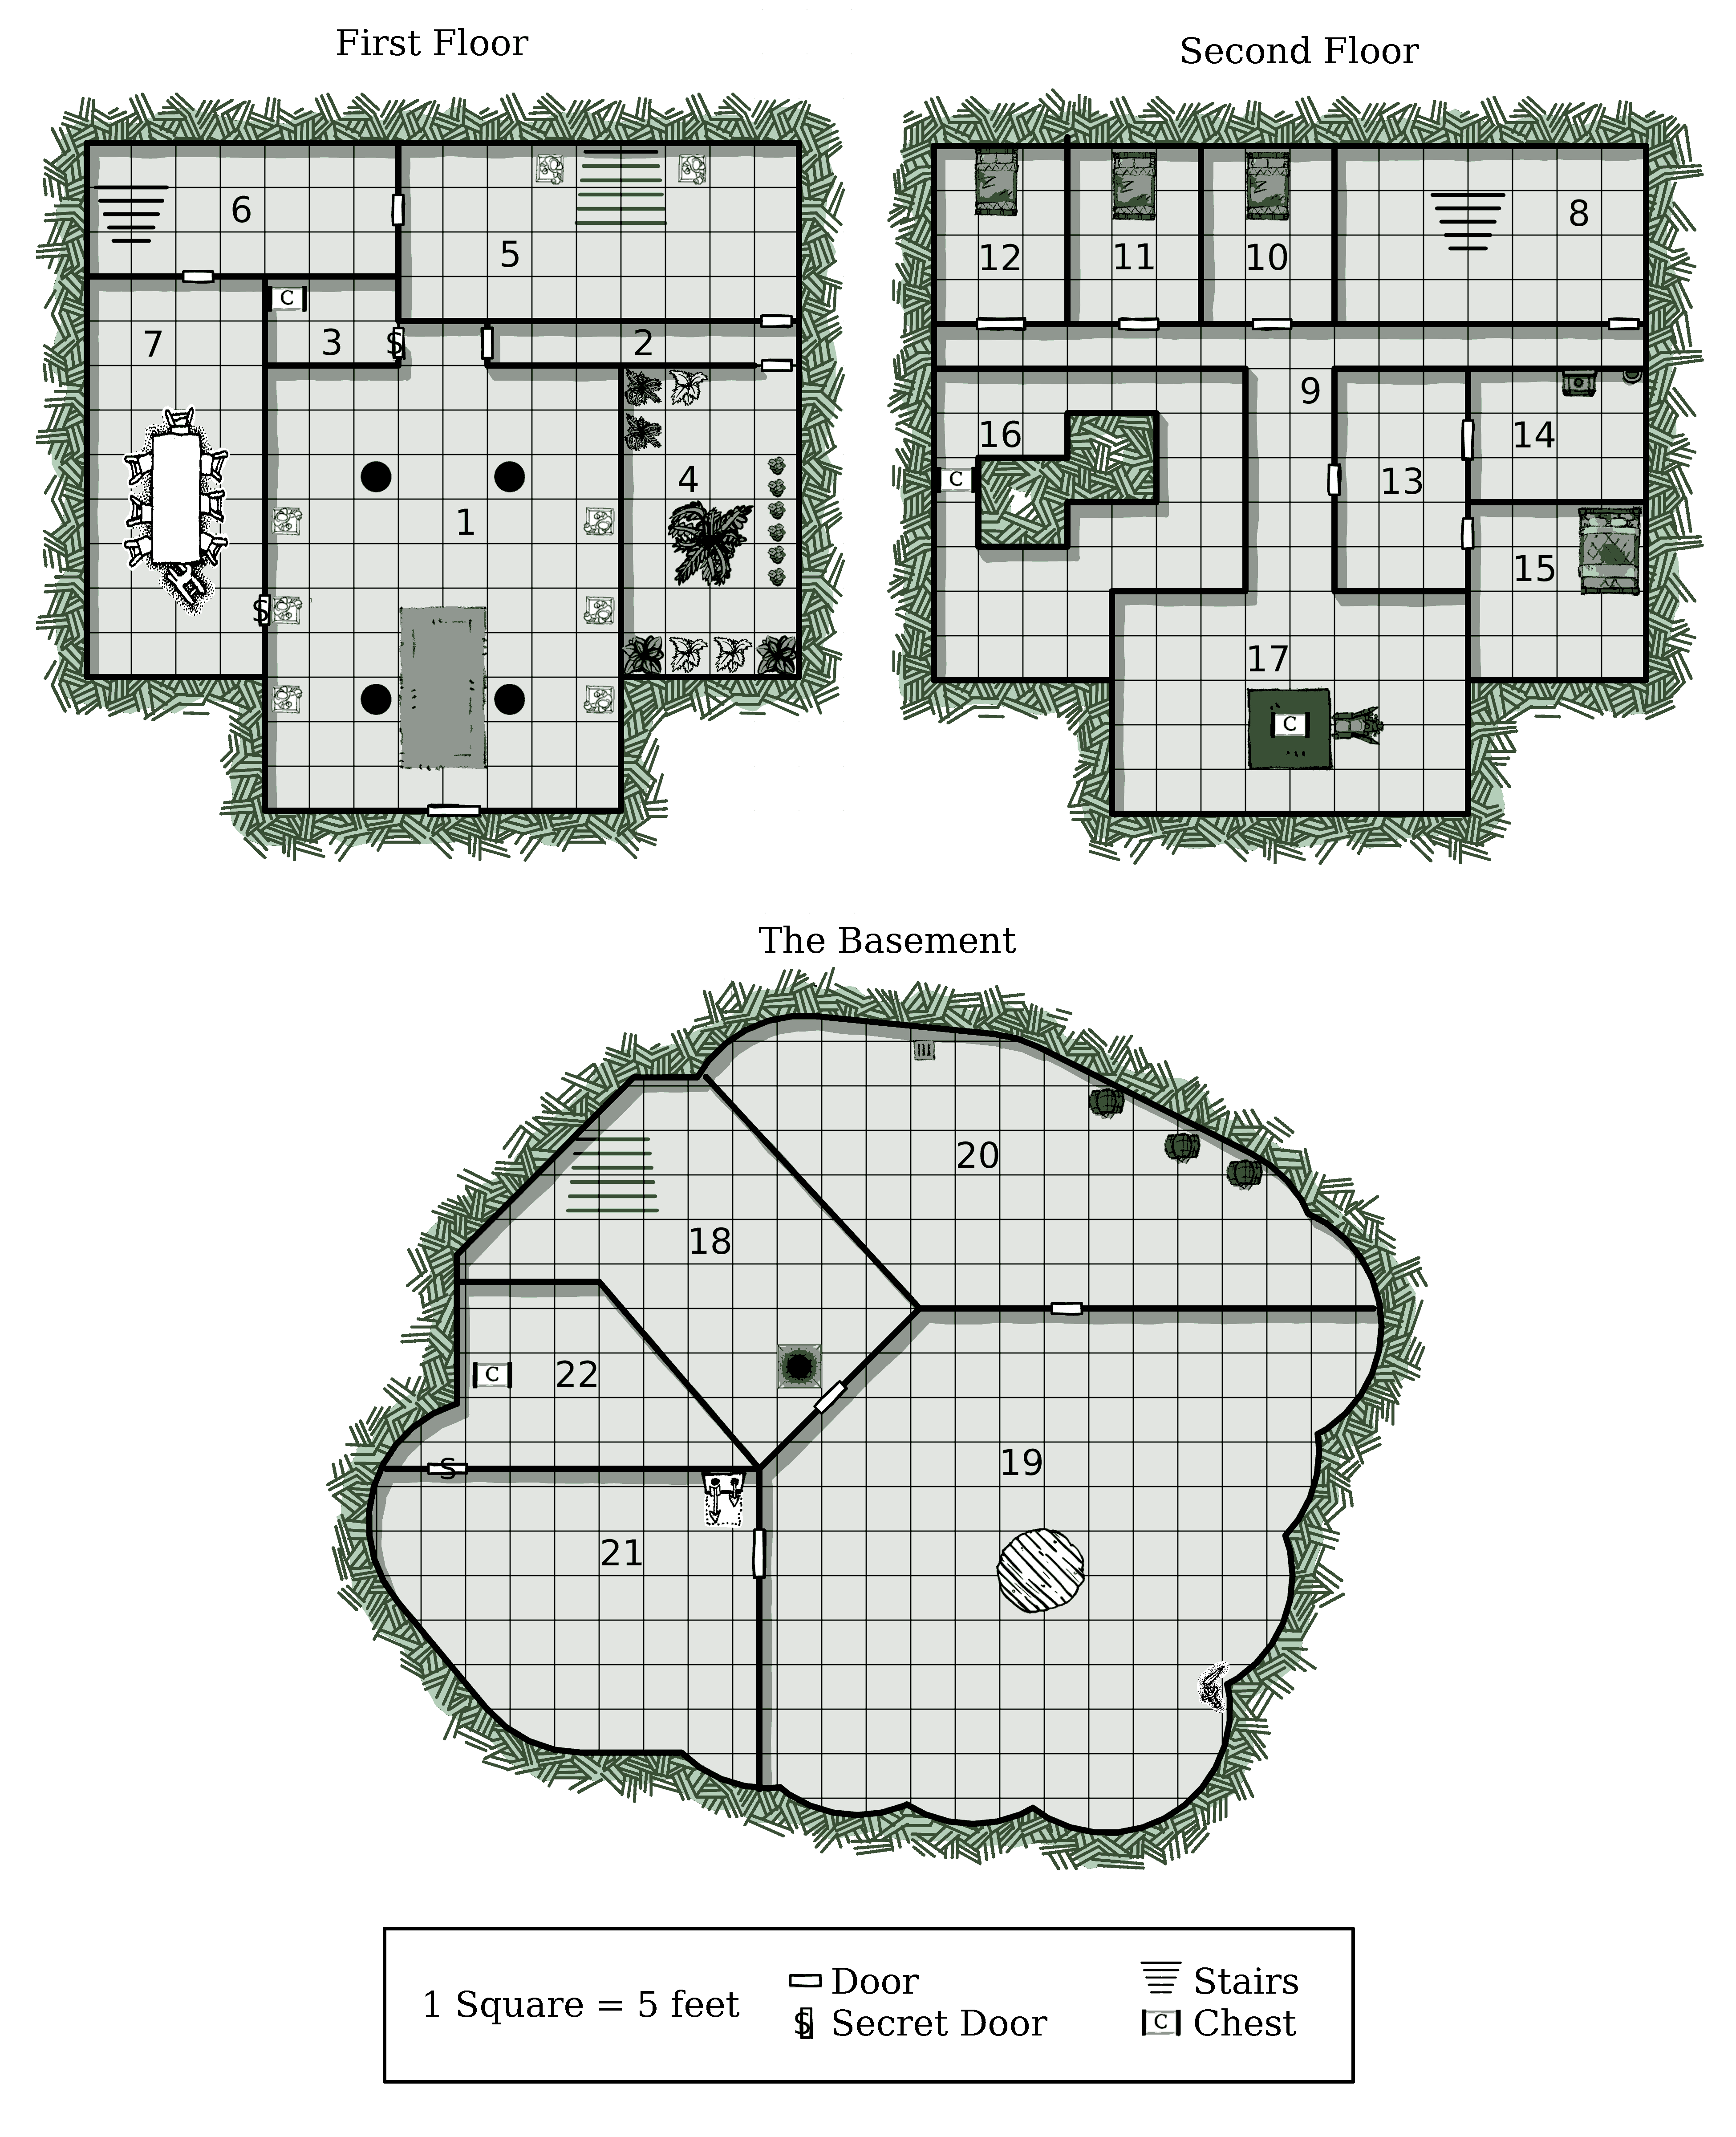
\includegraphics[width=\textwidth,height=0.9\textheight]{img/maps/ShakarrsMansion_45x45.png}
  \caption{Map 3.1 Shakarr's Vanishing Mansion}
\end{figure*}
\subsection{Conclusion}
The player's have explored the Vanishing Mansion of Shakarr. They are disappointed to not meet with the rumored wizard, and will have to continue in their voyages to search for intel about Amberia's brand. \\
Hopefully the players explored and were able to get some information about the world. By reading the notes in the Study, they should have received a clue that the owner of the mansion is connected to the Council of Seven. They could have learned about one of Malmalor Lumena's Curses, where she sabotaged one of Shakarr's experiments with time. They could have also gotten some foreshadowing about how Shakarr's memories are addled and out of order in time, which is why he recognizes them and runs away from them to begin with. And if they were very fortunate, they may have heard whispers of the underdark dwelling minions of the aberroth.\\
In the end, this dungeon should have provided the party with enough XP to reach Level 3, which should allow them to comfortably proceed on to the next adventure.
\section{The Aftermath}
The people of Garon City will be confused, but also relieved to see that the mansion that appeared one day has now disappeared just as suddenly, seemingly without causing them harm. Any townsfolk that recognize the party as adventurers might ask them about it. \\
If the party continue to ask around town for intel, the townsfolk should make it clear that they have no further information and encourage the party to seek the experts in Gold City.
